\documentclass[conference]{IEEEtran}
\IEEEoverridecommandlockouts
% The preceding line is only needed to identify funding in the first footnote. If that is unneeded, please comment it out.
\usepackage{cite}
\usepackage{amsmath,amssymb,amsfonts}
\usepackage{algorithmic}
\usepackage{graphicx}
\usepackage{textcomp}
\usepackage{xcolor}
\usepackage{graphicx}
\def\BibTeX{{\rm B\kern-.05em{\sc i\kern-.025em b}\kern-.08em
    T\kern-.1667em\lower.7ex\hbox{E}\kern-.125emX}}

\graphicspath{{images/}}
\begin{document}

\title{Secure, Private and Resilient Distributed Neural Network Deployments}

\author{\IEEEauthorblockN{Tollan Berhanu}
\IEEEauthorblockA{\textit{M.S. Computer Science} \\
\textit{University of Idaho}\\
Idaho Falls, ID, United States \\
January 2025}
}

\maketitle

\begin{abstract}
% Deep Neural Networks (DNNs) have emerged as foundational tools across diverse applications such as computer vision and natural language processing. However, the growing complexity and resource demands of modern DNNs pose significant challenges for real-time inference, particularly on resource-constrained devices. Distributed inference offers a solution by partitioning DNNs and distributing computational workloads across networks of devices, including edge nodes, cloud servers, and hybrid systems. (Say something about the security measures taken towards securing DDNNs against several attacks such as reverse engineering, DDoS, ...)
% This survey explores various research works surrounding distributed inference of DNNs, focusing on the deployment architectures, network latency challenges, communication optimization strategies, security risks and the methodologies enabling distributed inference.
\end{abstract}


\section{Introduction}

Deep neural networks (DNNs) are the foundation of modern intelligent systems, enabling advances in computer vision, natural language processing, and speech recognition. However, the growing size and computational demands of DNNs present significant challenges in their training and deployment. Distributed Deep Neural Networks (DDNNs) have emerged as a solution, leveraging the computational resources of multiple devices—ranging from edge nodes to cloud servers—to handle the complexities of modern DNNs \cite{ashouri2020analyzing, abdi2023efficient}. By splitting computational tasks across a network of devices, distributed approaches address the limitations of centralized processing, such as high communication overhead and latency when transferring large volumes of raw data to cloud servers \cite{chinchali2018neural, yang2021cooperative}.

While distributed inference reduces latency and improves resource utilization, it also introduces significant security challenges and opportunities. Partitioning DNNs and distributing their computations across multiple devices can make the model more resilient to reverse engineering by attackers, as the complete model structure and parameters are not accessible from any single device \cite{sahu2021denni}. Moreover, distributing computations enables redundancy and fault tolerance, ensuring that even if a subset of devices is compromised or fails, the remaining devices can continue to provide inference capabilities, enhancing the resilience of the deployment infrastructure \cite{ashouri2020analyzing}.

This survey focuses on the security aspects of DDNNs, exploring how distributed architectures can mitigate threats such as model theft, adversarial attacks, and data breaches. It examines techniques for secure partitioning, communication, and fault tolerance, emphasizing the role of distribution in protecting sensitive data and model integrity. Furthermore, the survey highlights the dual nature of distributed approaches: while they can enhance security through obfuscation and redundancy, they also introduce vulnerabilities, such as risks from compromised nodes or malicious interference during communication \cite{abdi2023efficient, teerapittayanon2017distributed}.

% #######################################################################################

% \section{Existing Surveys}

% #######################################################################################


\section{Background}

Distributed deep learning in general can be divided into a training phase and a prediction or inference phase. The training phase is computationally intensive phase involves training a machine learning model by feeding it large datasets and updating it using a specific ML algorithm. The result of this phase is a trained model, which can then be deployed. The inference phase refers to using the trained model to make predictions on new data inputs and it requires less computing power than the training phase. Distributed inference involves partitioning a DNN model into multiple sub-models or partitions. These partitions are then distributed to different devices for execution. This partitioning can occur at different granularities, ranging from layer-wise partitioning, where individual layers are assigned to different devices, to fused-layer partitioning, where groups of layers are combined into larger blocks for distribution \cite{hou2022distredge, zhao2018deepthings}. In more complex approaches like receptive field-based segmentation, the model is partitioned based on the receptive fields of different layers. The choice of partitioning strategy impacts the communication overhead incurred in exchanging intermediate data between devices, which can be a significant bottleneck in distributed inference.

Deep Neural Networks (DNNs) are a type of artificial neural network characterized by multiple hidden layers, making them particularly effective for tasks such as image recognition, speech recognition, and natural language processing. These networks can be deployed on central servers or directly on edge devices or end devices like edge servers, automobiles, mobile phones and IoT devices, depending on the use case. To maximize efficiency and scalability, distributed deep neural networks (DDNNs) are often deployed across a computing hierarchy that may include end devices, edge servers, and cloud platforms. This layered structure enables the flexible distribution of computational workloads \cite{chinchali2018neural, teerapittayanon2017distributed}.

Distributing neural networks primarily involves partitioning a large model into smaller sub-models or partitions, which are then assigned to different devices for parallel execution. This partitioning allows leveraging the combined processing power of multiple devices to accelerate inference, particularly beneficial in edge computing environments where devices often have limited resources. Techniques like model compression and early exit strategies further enhance the feasibility of distributing neural networks by reducing the model size and computation demands, while considerations for communication overhead, synchronization, resource heterogeneity, and model accuracy play a crucial role in choosing the optimal partitioning and distribution strategy for a specific application \cite{zhao2018deepthings}.

% Edge computing offers a compelling approach to support DDNN inference by moving computation closer to the data source. This approach not only reduces latency but also addresses privacy concerns by limiting the transfer of sensitive data to remote servers \cite{li2018edge, xue2020edgeld}. In a distributed inference system, multiple edge devices—or a combination of edge devices and more powerful edge servers or cloud resources—collaborate to execute DNN inference. Efficient communication between components in a DDNN is essential. Techniques such as layer fusion, inter-channel partitioning, and quantization are often employed to optimize this communication, ensuring minimal overhead and improved performance \cite{rodriguez2023horizontally}.

% The size and complexity of DDNNs, along with the massive amounts of data they process, have led to challenges in their training and deployment. Despite these challenges, these systems hold immense potential in various applications. They enable the deployment of complex DNN models on resource-constrained edge devices, facilitating intelligent applications in domains such as smart homes, smart factories, and smart cities. The ability to distribute computations across multiple devices not only improves inference speed but also enhances fault tolerance and redundancy \cite{sahu2021denni, zeng2020coedge}. Moreover, distributed inference can mitigate security and privacy concerns by distributing the model parameters across multiple devices, making it more difficult for attackers to reverse engineer the entire model.

% More about the security challenges in DDNNs


% #######################################################################################



\section{Motivations}

A key motivation for distributing neural network inference is to leverage the computational power of multiple devices, including edge servers, cloud platforms, and end devices. DNN partitioning enables the distribution of computation across a hybrid system of mobile devices and cloud platforms \cite{zhang2020towards, zhang2021deepslicing, li2018edge}. In this paradigm, a DNN model is divided into multiple parts and each part is assigned to a different device for execution. This distribution of workload allows for faster inference, as well as reduced energy consumption on resource-constrained devices \cite{zeng2020coedge, yun2022cooperative}. Distributing inference tasks within a manageable range also provides advantages in real-time response and data privacy preservation \cite{zeng2020coedge}.

Another primary motivation driving the research in distributed inference is the desire to reduce the execution latency of deep learning models. This is particularly important for applications that demand real-time responsiveness, such as self-driving cars and other intelligent applications in the edge computing paradigm. Traditional methods of accelerating DNN inference have focused on techniques like model sparsification and feature compression. Model sparsification involves pruning unimportant network parameters to reduce computation and memory requirements. This can involve both unstructured pruning, which removes individual parameters, and structured pruning, which prunes entire weight tensors to maintain compatibility with off-the-shelf hardware \cite{zou2021cap}. Feature compression aims to reduce the volume of intermediate data transmitted between devices during distributed inference \cite{zhang2021communication}. However, these techniques often introduce a trade-off between inference accuracy and speedup. The choice of model sparsity level and feature compression ratio significantly impacts both the computation workload and communication overhead, making finding the optimal balance a significant challenge.

Another key motivation is the need to support the increasing scale and complexity of DNN models. As DNN models grow in size, they become increasingly difficult to deploy on single devices, especially resource-limited ones. The growing demand for more complex DNN models further complicates this issue, pushing researchers to explore distributed inference as a means of leveraging more powerful hardware like cloud servers and edge clusters.

% A key motivation for distributed inference research stems from the inherent limitations of edge devices in terms of computational power, memory capacity, and energy budget. DNN inference, particularly for complex models, demands substantial computational resources, often exceeding the capabilities of individual edge devices. 

% Offloading these computationally intensive tasks to more powerful servers in the cloud or edge data centers introduces significant latency due to data transmission over wide-area networks. This latency bottleneck hinders the feasibility of real-time applications that rely on timely inference results.

Researchers are driven to explore distributed inference as a means of leveraging the collective resources of multiple edge devices and servers to overcome these limitations. By partitioning a DNN model and distributing its execution across a network of devices, the computational workload can be shared, reducing the burden on individual devices and potentially achieving faster inference speeds. This distributed approach also enables the utilization of more powerful edge servers or cloud resources for processing complex DNN layers, further enhancing inference capabilities.


% A primary motivation for distributed neural network inference is to enhance the performance of DNN-powered applications on resource-constrained devices. By strategically partitioning DNN models and distributing the computation across a hybrid system, developers can exploit the heterogeneous resources available in a distributed environment. This approach can significantly reduce the computational burden on individual devices, allowing for real-time or near real-time inference, even on devices with limited processing capabilities \cite{wu2022hitdl, xu2022eop}. Furthermore, distributing inference tasks can enhance data privacy by processing sensitive information locally on end devices while selectively offloading intermediate results to more powerful devices for further processing \cite{shao2020communication}.



% #######################################################################################


\section{Related Work}
% Related work on surveys regarding security and privacy related attacks on ML Models


% #######################################################################################

% \begin{figure*}[t]
%     \centering
%     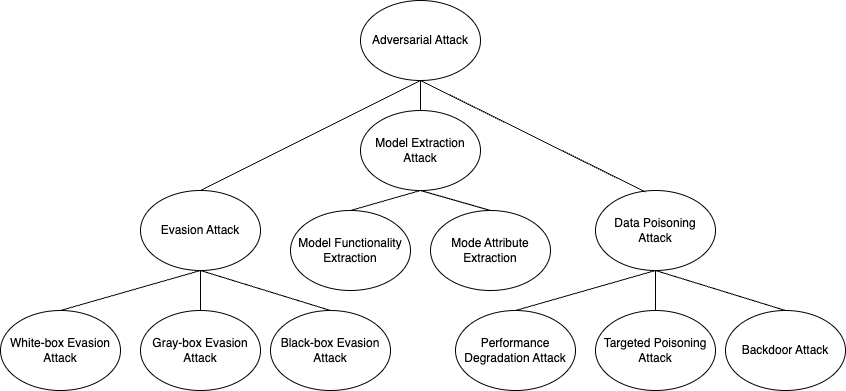
\includegraphics[width=\textwidth]{taxonomy2.png}
%     \caption{Taxonomy of Adversarial Attacks on ML Models}
%     \label{fig:taxonomy}
% \end{figure*}

\section{Attacks}
% Attacks on Non-distributed and Distributed Deep Learning Models

There are various types of attacks that can be performed on machine learning (ML) and deep learning (DL) models. These attacks can occur at different stages of the machine learning life-cycle, including the training and inference phases. The attacks can be broadly categorized into the following types (list all types / sub-types here):

% \subsection{Adversarial Attacks}
% Adversarial attacks on machine learning systems refer to deliberate attempts by malicious actors to compromise both the training and inference stages of a model, ultimately degrading its performance and reliability. During the training phase, attackers might launch poisoning attacks by introducing deceptive data samples or mislabeling inputs, which can skew the learning process. At the inference stage, adversaries often craft subtle, almost imperceptible perturbations to inputs—commonly known as adversarial examples—that lead the model to make incorrect predictions \cite{wu2021tolerating}. These vulnerabilities are particularly concerning in critical applications, such as autonomous driving or medical diagnostics, where even minor errors can have severe consequences. Adversarial attacks can be classified into three major categories: data poisoning attacks, evasion attacks and model extraction attacks.

% \subsection{Data Poisoning Attacks}
% Data poisoning attacks are a form of adversarial threat that target the training phase of machine learning models. In these attacks, adversaries intentionally inject, modify, or remove data in the training set to corrupt the learning process. This is especially critical in environments like Federated Learning, where multiple parties contribute data, often from untrusted sources \cite{sun2021data}.

% Data poisoning attacks can be broadly classified into several categories:

% \subsubsection{Performance Degradation Attacks:}
% The attacker introduces malicious examples into the training dataset with the aim of lowering the overall accuracy and robustness of the model. By contaminating the data, the adversary disrupts the model’s ability to learn accurate decision boundaries, resulting in widespread errors. For example, an attacker might inject anomalous network-layer protocol data into an intrusion detection system’s training set (labeled as normal) to degrade its detection capability \cite{pitropakis2019taxonomy}.

% \subsubsection{Targeted Poisoning Attacks:}
% Rather than affecting overall performance, targeted attacks are designed to cause specific misclassifications. Here, the adversary carefully selects or manipulates certain training samples (often through techniques like label-flipping) so that the model makes incorrect predictions on specific inputs during testing \cite{pauling2022tutorial}.

% \subsubsection{Backdoor (Trojan) Attacks:}
% In a backdoor attack, the adversary subtly implants a “trigger” or backdoor key into the training data. The model then learns to associate this trigger with a specific malicious behavior while performing normally on clean inputs. For instance, in an autonomous vehicle system, a backdoor could cause a stop sign to be misclassified as a speed limit sign when a specific mark is present on the sign \cite{chen2017targeted}.


\subsection{Model Evasion Attacks}
Model evasion attacks occur during the inference (or testing) phase of a machine learning model. In these attacks, the adversary subtly perturbs the input data to force the model into making incorrect predictions, without altering the model’s underlying training process. Typically, these perturbations are so slight that they remain undetectable to human observers, yet they exploit the weaknesses of the model in its decision boundaries \cite{golla2023security, pauling2022tutorial}.

For example, in a spam filtering system, an attacker might make minor modifications to spam emails so that they bypass the filter and are mistakenly classified as legitimate. This form of attack takes advantage of the fact that the deployed model, despite being well-trained, may still have vulnerabilities when exposed to inputs that lie near its decision boundaries.

Evasion attacks can be broadly categorized based on the level of knowledge the adversary possesses about the target model:

\subsubsection{White-box attacks:}
In a white-box scenario, the adversary has complete knowledge of the model, including its architecture, parameters and gradients \cite{ren2020adversarial}. This full transparency enables the attacker to compute precise perturbations (using methods such as the Fast Gradient Sign Method \cite{naqvi2023adversarial}, Projected Gradient Descent \cite{deng2020universal}, or the Carlini \& Wagner (C\&W) attack \cite{pujari2022approach}) that maximize the loss of the model on a given input. White-box attacks are typically the most effective because they directly exploit the internal workings of the model.

\subsubsection{Gray-box attacks:}
Gray-box attacks occur when the attacker has partial information about the target model. For example, the adversary may know the model architecture but not its exact parameters, or may have limited access to the output probabilities. This middle ground scenario allows attackers to approximate gradient information or leverage transferability from surrogate models, balancing realism with attack efficiency \cite{ren2020adversarial}.

\subsubsection{Black-box attacks:}
In a black-box attack, the adversary has no access to the internal structure or parameters of the model. Instead, they can only query the model and observe its outputs (such as predicted labels or confidence scores) \cite{ren2020adversarial}. Techniques in this setting include training a surrogate model to mimic the target model or using query-based methods (such as HopSkipJump \cite{newaz2020adversarial} or Square Attack \cite{andriushchenko2020square}) to estimate gradients indirectly. Although black-box attacks are often less efficient than white-box attacks, they more closely mirror real-world conditions, where internal model details are hidden.


\subsection{Model Extraction Attacks}
Model extraction attacks are designed to replicate or 'steal' the functionality, architecture, and sometimes its internal parameters of a target machine learning model. In these attacks, adversaries systematically query the target model - often deployed as a cloud-based API - with carefully chosen inputs to collect corresponding outputs. They then use these input-output pairs to train a substitute (or surrogate) model that closely mimics the behavior of the original model, effectively duplicating its decision-making process without direct access to its internal workings \cite{golla2023security}.

Model extraction attacks can be categorized based on the specific goals of the attacker \cite{gong2020model}:

\subsubsection{Model Attribute Extraction:}
This type of attack focuses on obtaining detailed information about the target model's internals, such as:
\begin{itemize}
  \item \textbf{Parameter Stealing:} Inferring the model's weights or other internal parameters by analyzing responses to carefully crafted queries.
  % \item \textbf{Hyperparameter Stealing:} Determining the hyperparameters used during training, which can reveal aspects of the model’s design and optimization process.
  \item \textbf{Architecture Extraction:} Reconstructing the model’s structure, including the number and type of layers, to understand its design.
  \item \textbf{Decision Boundary Inference:} Mapping the regions in the input space where the model’s predictions change, thereby approximating its decision boundaries.
\end{itemize}

\subsubsection{Model Functionality Extraction:}
Instead of recovering specific internal attributes, these attacks aim to duplicate the overall behavior of the target model. The attacker uses the gathered input-output pairs to train a substitute model that performs similarly to the target model on the same tasks. This type of extraction is often sufficient for many practical purposes, such as replicating service functionality or enabling further adversarial attacks.

% Techniques for Model Extraction
% Several techniques are employed to carry out model extraction attacks:
% Query-Based Attacks:
% The adversary sends a variety of inputs to the target model and records its outputs. The collected dataset is then used to train a surrogate model that approximates the target model's functionality.
% Optimization Techniques:
% Some approaches formulate the extraction process as an optimization problem. The attacker minimizes the difference between the outputs of the target model and the substitute model—often by solving for the model parameters that best replicate the observed responses.
% Meta-Model Training:
% In certain cases, attackers may build higher-level meta models that leverage theoretical equations or prior knowledge about typical model structures to guide the extraction process.

Model extraction attacks are particularly concerning for cloud-based ML services, where models are accessible via public APIs. The ease of querying these models (often with rich output such as probability scores) enables adversaries to reconstruct models that can then be used for further exploitation or competitive advantage \cite{gong2020model}.

% ############### Other classifications yet to be included in the taxonomy ###############

\subsection{Model Inversion Attacks}

Model inversion attacks focus on extracting sensitive information about the training data by exploiting the responses of a deployed model. Unlike model extraction, which aims to replicate the model’s properties, model inversion attacks are designed to reveal private attributes or even reconstruct portions of the original training data, thereby compromising user privacy \cite{dibbo2023sok}.

The primary goal of model inversion attacks is to infer confidential data that was used to train the model. For example, in a facial recognition system, an adversary might leverage confidence scores and output probabilities to reconstruct a recognizable image of an individual. Attackers achieve this by carefully selecting input queries and analyzing the model's responses. The amount of information leaked often depends on how over-fitted the model is and the granularity of the output it provides.

Model inversion attacks can be organized into two primary categories:

\subsubsection{Inference Attacks}
These attacks focus on deducing sensitive attributes or properties of the training data without necessarily reconstructing the full data instance. They include:

\paragraph{Attribute Inference:}
The adversary exploits output labels, confidence scores, and auxiliary information to infer exact values of sensitive attributes from individual data samples. For instance, given partial information about a customer, the attacker may accurately predict their credit score or medical condition.

% \paragraph{Approximate Attribute Inference:}
% In these attacks, the adversary does not recover the exact attribute value but instead obtains an approximation that is close enough to reveal private information.

\paragraph{Property Inference:}
Rather than targeting a specific attribute, property inference attacks aim to deduce general properties or trends in the training data. For example, an attacker might determine if a dataset predominantly consists of images of people wearing glasses, without reconstructing any specific individual’s image.
\setcounter{paragraph}{0}

\subsubsection{Reconstruction Attacks}
These attacks attempt to rebuild data samples from the training set. 
These attacks target distributed ML models by attempting to reconstruct private input data samples from the intermediate representation leaked by edge devices. The most notable reconstruction attack is image reconstruction attack. Attackers can query the model with chosen images and use the image intermediate representation pairs to train a reconstruction model \cite{benkraouda2021image}. Image reconstruction attacks are further subdivided into:

\paragraph{Typical Image Reconstruction (TIR):}
The adversary reconstructs a generic or average image that represents the learned characteristics of a particular class. This gives insight into the overall features captured by the model \cite{dibbo2023sok}.

\paragraph{Individual Image Reconstruction (IIR):}
More targeted than TIR, these attacks focus on reconstructing a specific individual’s image from the training data. Such attacks pose a significant privacy risk as they can lead to the exposure of personally identifiable information \cite{dibbo2023sok}.
\setcounter{paragraph}{0}



% \subsection{Byzantine Attacks}
% Byzantine attacks present a serious threat to distributed and federated learning systems. These attacks occur in distributed machine learning systems, where some workers are compromised and send malicious gradients to the parameter server, leading the training process to a wrong model \cite{wu2021tolerating}. In these attacks, one or more nodes behave in a malicious or faulty way. Instead of contributing valid updates to the model, these nodes send deceptive, arbitrarily altered, or even colluding updates that can undermine the entire training process. The goal is to manipulate the global model, steering it away from optimal performance and degrading its overall accuracy and reliability. Even a single malicious node can have a significant impact on the performance of the model. In some cases, the model’s accuracy can drop dramatically from near-perfect performance to complete failure due to the influence of these malicious updates. The global model may no longer generalize well or even fail to learn anything meaningful \cite{shi2022challenges}.

% One of the defining features of Byzantine attacks is that they are executed by nodes that do not follow the prescribed protocol. These nodes could either be inherently faulty or actively malicious. When they send updates, such as gradients or model weights, these updates differ drastically from those sent by the honest participants in the system. This deviation can significantly disrupt the training process and prevent the model from learning effectively \cite{konstantinidis2023detection}. Unlike other types of attacks that occur during inference, Byzantine attacks specifically target the training phase of machine learning. In a typical distributed learning setup, local updates from individual nodes are aggregated at a central server. If a malicious node sends corrupted updates, it can distort the aggregation process, thereby impacting the global model and making it unreliable \cite{wang2021elite}.

% Attackers can manipulate the updates in several ways to disrupt the training. The attacker may deliberately flip the sign or adjust the magnitude of the gradients, aiming to mislead the optimization process and steer the model in the wrong direction. The attacker may also introduce random noise into the updates, which can disturb the model’s convergence and slow down or halt progress if done strategically \cite{shi2022challenges}. This makes the detection of Byzantine behavior to be notoriously difficult. Malicious nodes may behave in ways that mimic legitimate participants, or they might adapt their strategies over time to avoid detection. In cases of colluding attacks, where multiple nodes work together to disrupt the model, it becomes even harder to identify the malicious intent. The coordinated actions of several malicious nodes can easily mask their behavior, making it challenging for the system to pinpoint and mitigate the attack \cite{shi2022challenges, wu2021tolerating}.



% \subsection{Model-Reuse Attacks}
% Model-reuse attacks occur when maliciously designed models are used to cause a host machine learning system to misbehave on specific inputs. These malicious models are crafted to misclassify targeted inputs while appearing harmless on non-targeted ones. Such attacks typically happen when developers reuse pre-trained models from untrusted sources. They exploit the common practice of building complex ML systems by integrating pre-trained models, which are usually tailored for tasks like feature extraction \cite{ji2018model}.



% #######################################################################################



\section{Methodologies and Approaches}

Several studies have explored the security vulnerabilities of distributed deep neural networks (DNNs) in resource-constrained environments. Two major attack vectors have been identified: side-channel attacks on compressed communication and Trojan-based attacks on distributed convolutional neural networks (CNNs). These attacks exploit different weaknesses in distributed inference systems and require distinct countermeasures.

\subsection{Threat Model}
\cite{kannan2024security} focuses on side-channel vulnerabilities in Distributed Deep Neural Networks (DDNNs) that use compressed communication between edge devices and central servers. The paper demonstrates that an attacker can infer the DDNN’s output by observing the size of encrypted compressed messages. Two attack methods, Gaussian Likelihood and Rank Order Decision Trees, successfully exploit this vulnerability, achieving over two times the accuracy of random guessing in both white-box and gray-box attack settings.

\cite{mohammed2020secure} investigates Trojan-based attacks on distributed CNNs running across multiple IoT edge devices. The proposed attack model assumes an adversary controls a single compromised node within the distributed system. Five attack strategies modify CNN layer parameters, including scaling, random perturbations, polarity flipping, max-min swaps, and statistical weight replacement. These stealthy attacks degrade classification accuracy without altering the overall CNN structure, making them difficult to detect.

\subsection{Defense Strategies}
To defend against side-channel attacks on compressed communication, \cite{kannan2024security} introduces Dropout Stable Compression (DRSC). DRSC eliminates message size variability by dropping near-zero values before compression, ensuring fixed-length encrypted messages. This method effectively prevents side-channel inference while maintaining inference accuracy within 0.3\% of standard compression methods. DRSC also incurs negligible computational overhead, making it suitable for resource-constrained edge devices.


% #######################################################################################

\section{Applications of Distributed Deployments}

Distributing machine learning computations among various devices and network layers is rapidly transforming the deployment of intelligent systems, especially in edge computing environments. Processing data near its source mitigates computational latency constraints and strengthens data privacy and security, as sensitive information remains on local devices rather than being transmitted to centralized servers. There are several applications of distributed inference of models. Some notable applications include autonomous vehicles, IoT and healthcare systems.

% One prominent application is in intelligent mobile applications. Mobile devices, constrained by limited processing power, often struggle with resource-intensive DNN tasks such as image and speech recognition. While offloading these tasks to the cloud can introduce variable latency and potential security risks, distributed inference splits the computation between mobile devices and nearby edge servers. This setup enables real-time performance for applications like image recognition \cite{li2018edge} and speech recognition \cite{bhattacharya2016sparsification, zou2021cap}, while incorporating secure data handling and encrypted communication to safeguard user information. Such measures are critical for augmented reality and interactive applications, where immediate and trusted responses are essential \cite{liu2021eeai, zeng2020coedge}.

% In the Internet of Things (IoT) domain, distributed inference is vital for processing large volumes of data generated by devices in scenarios like environmental monitoring, smart home automation, and industrial sensor analysis. By partitioning inference tasks across multiple devices, these systems not only overcome the limitations of single-device execution but also integrate security measures—such as encryption of intermediate outputs and secure multi-party computation—to prevent data tampering and unauthorized access \cite{xue2020edgeld, naveen2021low}.

\subsection{Applications of Distributed Inference in Autonomous Vehicles}

Autonomous vehicles (AVs) leverage distributed inference to rapidly process vast amounts of sensor data, including video streams and radar signals, to support real-time decision-making. Computationally intensive tasks like object detection and scene understanding are delegated to edge servers, while critical low-latency processes remain on-board. \cite{mohammed2020distributed}. Distributed inference is critical in enabling AVs, from ground vehicles to aerial drones, to perform complex tasks with real-time responsiveness. In unmanned aerial vehicles (UAVs), distributed inference facilitates critical surveillance applications such as wildfire detection, infrastructure inspection, and threat identification in military zones. UAV swarms capture high-resolution images and process them collaboratively using CNNs, avoiding reliance on remote servers. For instance, the OULD framework \cite{jouhari2021distributed} dynamically partitions CNN layers across UAVs to classify captured images onboard, enabling rapid incident detection in environments with unstable connectivity. 

In autonomous cars, distributed inference involves partitioning models across end devices (onboard Electronic Control Units (ECUs)), edge nodes, and cloud servers, enabling AVs to perform complex tasks such as environment perception, path prediction, and real-time decision-making efficiently. For instance, environment perception tasks, including object detection and scene segmentation, often utilize convolutional neural networks (CNNs) to process inputs from cameras and LiDAR sensors \cite{mohammed2020distributed}. Similarly, recurrent neural networks (RNNs) are deployed for temporal tasks like Most Probable Path (MPP) prediction, which anticipates a vehicle’s trajectory based on historical GPS data and map context \cite{grigorescu2020cloud2edge}. These applications demand low-latency processing to ensure real-time responsiveness, necessitating distributed frameworks that balance computational load across multiple nodes.

\subsubsection{Methods of Distributing Models in AVs}

Distributed inference in AVs often involves partitioning DNNs and allocating computations across multiple computing nodes, such as edge devices and central servers. A prominent approach includes adaptive DNN partitioning and offloading, where tasks are split into finer-grained segments, smaller than a single layer, and processed collaboratively by devices in a network. This method balances computational loads between nodes while minimizing latency \cite{mohammed2020distributed}.

The Distributed Inference Acceleration (DINA) framework \cite{mohammed2020distributed} partitions DNNs into fine-grained sub-tasks, allowing layers or even sub-layers to be processed locally on edge devices or offloaded to fog/cloud nodes. This partitioning is optimized using a load balancing algorithm that dynamically assigns tasks to nodes based on network conditions, computational capacity, and queuing delays. The Cloud2Edge Elastic AI Framework \cite{grigorescu2020cloud2edge} follows a similar approach, where training and inference tasks are elastically distributed between cloud servers and edge ECUs. Sensitive data is pre-processed locally on edge devices to ensure privacy and reduce cloud dependency, while non-sensitive tasks leverage cloud infranstructures. 

Distributed inference in UAVs introduces unique methodologies related to to aerial mobility and resource constraints of UAV processors. The optimal UAV-based layer distribution (OULD) framework \cite{jouhari2021distributed} places CNN layers across UAVs to minimize latency. In order to avoid frequent re-allocation of inference tasks, the framework employs mobility prediction (OULD-MP), which anticipates UAV trajectories to preemptively adjust task allocations. UAVs prioritize air-to-air communication quality, to mitigate path loss and interference. Additionally, UAV frameworks avoid cloud dependency by preprocessing data locally and handle dynamic topologies by swarm coordination. For example, Raspberry Pi-equipped UAVs execute lightweight CNN segments, while deeper layers are offloaded to neighboring drones.


\subsubsection{Motivations for Distributing Models in AVs}

The primary motivations for distributed inference in self-driving cars include latency reduction, computational efficiency, and privacy preservation. Offloading compute-intensive tasks to nearby fog nodes or the cloud reduces latency for operations like object detection, which is critical for safety in AVs \cite{mohammed2020distributed}. Additionally, distributing models addresses the computational limitations of embedded ECUs, which lack the resources to execute large DNNs independently. Finally, privacy concerns are addressed through techniques like differential privacy (DP) and federated learning, which ensure sensitive data remains on local devices \cite{grigorescu2020cloud2edge}.

Distributing inference in UAVs is driven by the need for real-time responsiveness and operational reliability in harsh environments. Unlike autonomous vehicles, which offload tasks to fog/cloud nodes \cite{mohammed2020distributed}, UAVs often operate in remote areas (e.g., forests, offshore sites) where cloud connectivity is unreliable. Local processing reduces latency by avoiding data transmission to distant servers which is critical for time-sensitive tasks like wildfire detection. Furthermore, UAV swarms optimize bandwidth usage by transmitting only intermediate CNN outputs rather than raw images  \cite{jouhari2021distributed}. 


\subsubsection{Challenges for Distributing Models in AVs}

Despite its benefits, distributed inference in AVs face significant challenges. In self-driving cars, the main challenge is deciding how to collaboratively partition and distribute computations under continuously changing network conditions, such as fluctuating bandwidth and intermittent connectivity, which complicate task offloading decisions \cite{mohammed2020distributed}. Communication overhead can also be a major challenge as continuously transmitting data between edge devices can cause network delays. In the context of UAVs, dynamic network conditions can be caused due to their mobility, altitude changes and environmental interference, requiring real-time adjustments to inference task allocation. Additionally, air-to-air communication bottlenecks arise from limited bandwidth and interference in dense swarms, which in turn increase transmission delays between nodes \cite{jouhari2021distributed}.



\subsection{Applications of Distributed Inference in IoT devices}

Distributed inference in IoT and edge computing enables ML models to be executed closer to the data source, a capability that is critical in environments such as smart cities and industrial settings. In smart cities, for instance, the deployment of distributed inference allows data from smart cameras and environmental sensors to be processed locally. This local processing reduces both latency and bandwidth usage, which is critical for real-time surveillance, object detection, facial recognition, and anomaly detection in security systems. This also results in improved privacy, as sensitive data need not be transmitted over long distances to centralized data centers \cite{grzesik2024combining}.

In industrial IoT (IIoT) applications, distributed inference is deployed to support functions such as predictive maintenance, quality control, and anomaly detection. Here, the collaboration between resource-constrained sensors and more capable edge servers creates a system that can analyze massive data streams in near real time. For example, in a smart manufacturing environment, inference tasks may be divided between a compressed model running on an IoT device and a full, high-accuracy model hosted on an edge node, allowing the system to dynamically adjust data sampling rates and offload computational tasks as network conditions change \cite{grzesik2024combining}.

\subsubsection{Methods of Distributing Models in IoT devices}

Distributed inference in IoT and edge computing leverages a combination of hardware platforms, software frameworks, and algorithmic strategies to deploy ML models across edge devices, fog nodes, and cloud servers. The methods used for distributing machine learning models across the edge involve several key strategies. One common approach involves model partitioning, where DNNs are split into segments that are distributed between edge devices and central nodes.  \cite{filho2022systematic, grzesik2024combining}. This partitioning enables lower-complexity models to run on constrained devices while offloading more computationally intensive tasks to nearby edge servers.

Frameworks like TensorFlow Lite and PyTorch Mobile optimize models for edge deployment through techniques such as model pruning and quantization to further reduce the computational overhead \cite{zhang2020deep}. Federated learning is another key method, where models are trained collaboratively across distributed edge nodes without sharing raw data, therefore preserving privacy of individual nodes. Before these models are deployed, they can be trained using federating learning methods, where each node participates in the training process, or they can be trained centrally and then deployed to the edge where they continue to operate independently. The latter case is commonly seen in applications where the training phase is handled in a controlled environment before the model is offloaded to IoT units \cite{filho2022systematic}.

% In decentralized multi-agent systems, edge devices collaborate to share model updates based on data gathered locally. For example, in smart cities, distributed cameras might offload computation to neighboring nodes to balance workloads, while IIoT systems use hierarchical causal graphs to predict equipment failures \cite{sedlak2024active}.


\subsubsection{Motivations of Distributing Models in IoT devices}

The motivations behind distributing these models stem primarily from the need to minimize latency, reduce bandwidth and preserve user privacy. As edge devices become more powerful because of advancements like integrated AI chipsets and hardware accelerators, the feasibility of running sophisticated models on the edge has increased \cite{grzesik2024combining}. Furthermore, the decentralized architecture inherently enhances system scalability and resilience by reducing the load on centralized servers and allowing each edge node to operate independently.

The primary motivation for distributing ML models lies in addressing the limitations of centralized cloud processing. Reducing latency is critical for time-sensitive applications like real-time surveillance systems, where distributed inference ensures immediate decision-making abilities \cite{grzesik2024combining}. For example, smart cameras performing facial recognition or anomaly detection rely on local processing to avoid delays caused by sending large volumes of data to centralized clouds \cite{filho2022systematic}. Bandwidth conservation is another driver, particularly in IIoT environments where high-frequency sensor data would overwhelm network resources if transmitted in full to the cloud \cite{grzesik2024combining}. Distributed systems also enhance data privacy, as sensitive information can be processed locally \cite{filho2022systematic}. Additionally, edge deployment ensures offline functionality in remote or unreliable connectivity scenarios, such as environmental monitoring in secluded areas \cite{grzesik2024combining}.
% Distributed inference also enhances scalability and resilience; for example, elastic edge systems autonomously scale resources to maintain Quality of Service (QoS) during peak demand \cite{sedlak2024active}.


\subsubsection{Challenges of Distributing Models in Industrial Applications}

Distributing ML models introduces significant challenges. Resource constraints on edge devices, such as limited computational power, memory, and energy, necessitate highly optimized models, often at the cost of reduced accuracy \cite{filho2022systematic, grzesik2024combining}. For instance, compressing models via quantization or pruning may degrade the model's performance. Heterogeneity across edge devices, such as varying hardware capabilities, operating systems, and communication protocols, complicates the distribution as models trained for one edge node may not generalize to others. Furthermore, all the nodes may not be able to handle the same amount of computational tasks. \cite{grzesik2024combining}. As distributed systems expand, security risks persist requiring robust encryption and authentication mechanisms to protect model updates and data \cite{filho2022systematic}. Communication inefficiencies further challenge distributed inference because synchronization delays between nodes or model partitioning can be a bottleneck to real-time applications \cite{filho2022systematic}. Finally, scalability remains a concern, as managing thousands of edge nodes in smart cities or IIoT environments demands adaptive orchestration frameworks to balance workloads dynamically \cite{grzesik2024combining}.

% The power sector, especially power distribution networks (PDNs), is exploring distributed inference to improve system reliability. As the volume of data from edge devices in complex PDNs increases, real-time data fusion and analysis become essential for stabilizing energy flow and ensuring control reliability. Advanced security measures, including encrypted data transmission, secure routing, and intrusion detection, are integral to these systems, protecting critical infrastructure from cyber-attacks \cite{luo2021cloud}.

% Beyond these examples, distributed inference is instrumental in smart cities—supporting video analytics for traffic management, public safety, and environmental monitoring—and in retail, where it powers personalized recommendations and customer behavior analysis. In both cases, the decentralized architecture not only enhances responsiveness and scalability but also embeds robust security measures to protect critical data and ensure regulatory compliance.

\subsection{Applications of Distributed Inference in Healthcare Systems}

Distributed inference has transformative applications in healthcare. By leveraging local, edge, and cloud-based resources, distributed inference systems can process sensitive health data closer to its source, reducing latency and enhancing privacy. In medical imaging, for instance, distributed architectures accelerate the analysis of MRI and CT scans, enabling faster diagnostics and treatment planning. Wearable devices, such as smartwatches, utilize on-device inference to monitor vital signs like ECG and oxygen levels in real time. In drug discovery, distributed computing frameworks parallelize complex simulations, such as protein folding, to expedite research and development.

\subsubsection{Methods of Distributing Models in Healthcare Systems}

Distributed inference in healthcare employs various strategies to deploy machine learning models across multiple computing tiers. One common method involves partitioning models across local, edge, and cloud tiers. In medical imaging, such as MRI or CT scan analysis, large datasets are processed by splitting workloads across multiple servers or cloud nodes using data parallelism, where subsets of images are analyzed concurrently. In this setup, lightweight preprocessing occurs on local nodes near data sources (e.g., MRI/CT scanners), while computationally intensive tasks like image reconstruction are offloaded to edge servers or cloud data centers \cite{akdemir2025technical}. 

For wearable devices, on-device inference enables real-time monitoring of metrics such as ECG or blood oxygen levels by deploying lightweight models directly on the hardware, which minimizes reliance on external servers. In several cases, on-device inference is prioritized to enable real-time health monitoring, such as detecting arrhythmias via ECG analysis directly on smartwatches \cite{al2022machine}. 

In drug discovery, distributed systems accelerate tasks like molecular simulations by utilizing high-performance computing clusters. Distributed computing clusters parallelize inference tasks to accelerate research, such as predicting protein folding structures, though this application often relies on high-performance computing frameworks beyond typical healthcare infrastructures. \cite{tuli2020healthfog}


\subsubsection{Motivations of Distributing Models in Healthcare Systems}

The primary motivation for distributing ML models in healthcare is to address critical constraints in latency, privacy, and scalability. In medical imaging systems, sensitive medical data should be processed locally or at the edge to minimize communication delays for time-sensitive diagnostics like real-time patient monitoring. Additionally, resource-constrained wearable IoT devices necessitates lightweight, localized models to enable low-latency processing \cite{al2022machine}. Privacy regulations also drive the adoption of edge and federated learning approaches, as sensitive data remains localized rather than being transmitted to centralized servers.

Distributed inference also addresses computational demands in drug discovery, where simulating complex molecular interactions requires scalable resources for parallel processing of massive datasets. Additionally, hybrid cloud-edge architectures balance workload distribution, ensuring resource-intensive tasks are offloaded to the cloud while time-sensitive analyses occur at the edge, optimizing both speed and cost.

\subsubsection{Challenges of Distributing Models in Healthcare Systems}

Despite its benefits, distributed inference in healthcare faces significant technical and regulatory challenges. Data heterogeneity—arising from varied sensor types, formats, and institutional protocols—complicates model interoperability \cite{akdemir2025technical}. For example, wearable devices from different manufacturers may produce inconsistent ECG signals. Regulatory compliance, imposes strict requirements on data privacy, as distributed systems must navigate varying data protection laws across regions. \cite{akdemir2025technical, tuli2020healthfog}. Resource constraints, including limited computational power on edge nodes and wearables, restrict model complexity, often necessitating trade-offs between accuracy and efficiency. Network reliability further challenges real-time applications, as unstable connections between tiers can delay critical diagnostics. Finally, synchronizing model updates across distributed nodes remains an issue, particularly in environments where data distributions may vary widely \cite{akdemir2025technical, al2022machine}.



% Overall, as distributed inference continues to evolve, its role in delivering real-time, resource-efficient, and privacy-preserving intelligent systems is becoming indispensable. Its broad applicability—from autonomous systems and IoT to healthcare, industrial automation, smart cities, and retail—is further enhanced by integrated security protocols that protect data at every stage of the inference process.



% #######################################################################################


\section{Security and Privacy Aspects of Distributed Deployments}

Deploying DL models in distributed environments offers significant security and privacy advantages, particularly during the inference stage. One privacy advantage of distributed model deployment is data localization. By design, distributed inference frameworks ensure that sensitive data remains fragmented across devices or edge nodes. For instance, RL-DistPrivacy \cite{baccour2022rl} partitions CNN feature maps across heterogeneous IoT devices, ensuring that no single device holds sufficient information to reconstruct the original input. This approach aligns with the principle of data localization, where only essential features are processed on the devices, and intermediate results are distributed among other nodes. Similarly, \cite{schlegel2022privacy} splits user data into shares processed by edge servers, ensuring that even if a subset of servers is compromised, the original data remains protected. These strategies minimize the attack surface for adversaries, as breaching a single node yields limited information about the overall dataset or model. 

From a security perspective, distributed ML deployment enhances resilience against targeted attacks. For example, another critical advantage lies in the reduced risk of centralized data breaches. Centralized systems, by their nature, present a single point of failure, where a breach could expose the entire dataset or model. By decentralizing data and computation across edge and server clusters, distributed models ensure that no single node holds complete knowledge of the model architecture or its parameters. For instance, RL-DistPrivacy ensures that IoT devices collaborate to compute inference tasks without exposing raw data to untrusted participants \cite{baccour2022rl}, while privateMDI distributes model parameters across edge server clusters, ensuring that no single server holds complete knowledge of the model \cite{dehkordi2024privacy}. This decentralization not only complicates adversarial efforts to reconstruct sensitive information but also limits the impact of a breach to isolated nodes or subsets of data.

Distributed systems also facilitate the integration of advanced privacy-preserving techniques, such as differential privacy (DP) and multi-party computation (MPC).DP provides a strong privacy guarantee for machine learning models. By introducing noise during training or inference, it reduces the ability of attackers to infer whether specific data points were in the training set. Therefore, distributed systems could further obscure individual contributions using DP, thereby ensuring their privacy. MPC strategy ensures that no single edge server or cluster can reconstruct the client’s data or the model's parameters, even if subsets of servers collaborate. The system’s threat model assumes semi-honest participants and tolerates collusion among up to a certain number of edge servers in a cluster. For example, \cite{dehkordi2024privacy} uses additive secret sharing and linearly homomorphic encryption to protect both model parameters and user data during inference. 


% #######################################################################################



\section{Challenges and Open Issues}

Distributed deep neural networks (DDNNs) offer significant potential for accelerating inference in edge computing environments. However, several challenges and limitations hinder their effective deployment, particularly in resource-constrained and heterogeneous settings. These challenges span model partitioning, latency prediction, communication overheads, resource management, and reliability, among others.

A key challenge is the limited applicability of current model partitioning techniques to complex neural network architectures. Popular methods such as QDMP, DADS, and Neurosurgeon work well for models represented as directed acyclic graphs (DAGs) but struggle with architectures that include loops, such as recurrent neural networks (RNNs), long short-term memory (LSTM) networks, and modern transformer-based models like BERT and XLNet. These architectures cannot be fully represented as DAGs, making it difficult to partition and deploy them effectively on distributed devices \cite{zhang2021dynamic, zhao2018deepthings, zhou2021dynamic}. Addressing this limitation is critical to expanding the usability of DDNNs.

Communication overheads in distributed systems further complicate efficient inference. Techniques like Structure-Level Parallelization (SLP) and Sparse Synaptic Weights (SSW) aim to reduce these costs but often fall short of fully exploiting optimization opportunities. For example, while Communication-Aware Automated Parallelization (CAP) has demonstrated promise using structured sparse activation and reinforcement learning, its application is hindered by the vast optimization space and the difficulty of identifying optimal solutions \cite{zou2021cap}.

Resource constraints, particularly memory limitations on edge devices, remain a persistent issue. Techniques like DeepThings' Fused Tile Partitioning (FTP) reduce memory usage by dividing computations into smaller units, but this often comes at the cost of reduced accuracy \cite{zhao2018deepthings}. Balancing memory efficiency and model performance remains a pressing need, particularly in dynamic IoT environments where data sources and system constraints frequently change \cite{mohammed2020distributed, naveen2021low}.

The heterogeneity of devices and fluctuating network conditions add further complexity to DDNN deployment. While strategies such as dynamic partitioning and network switching aim to mitigate these challenges, they often fail to adapt effectively under real-world conditions. Ensuring reliable performance across diverse hardware platforms and network environments requires robust, adaptive algorithms capable of responding to variability in real time \cite{karjee2022split, li2019edge}.


Finally, reliability and fault tolerance remain a critical challenge for distributed systems, especially in the context of DDNNs. Device failures, network disruptions, and synchronization challenges can severely impact system performance. Modular system designs with built-in redundancy and fail-safe mechanisms are essential to address these vulnerabilities \cite{zeng2020coedge}. Furthermore, integrating specialized hardware accelerators with optimized software frameworks is a promising approach for improving performance and energy efficiency, but this requires careful consideration of hardware constraints and software compatibility \cite{kress2022hardware, naveen2021low}.




% #######################################################################################




\section{Future Directions}

Future research on DDNNs should focus on overcoming the outlined challenges to enable more efficient and scalable systems. A primary area of focus is extending partitioning methods to accommodate non-DAG architectures, such as RNNs, LSTMs, and transformers, to expand the range of models suitable for distributed deployment \cite{zhang2021dynamic, zhao2018deepthings}. Additionally, advancing adaptive partitioning techniques that consider real-time resource availability, network conditions, and workload heterogeneity can significantly enhance the flexibility and efficiency of distributed systems. Research into optimizing latency prediction and resource allocation models is also crucial for ensuring real-time performance, particularly in applications requiring low-latency responses like autonomous driving and healthcare monitoring. Furthermore, exploring energy-efficient algorithms and lightweight architectures tailored for distributed environments can address the growing demand for sustainability in edge and IoT deployments.

% Another critical direction is the development of more accurate latency prediction models that incorporate framework-specific and hardware-specific factors, improving the reliability of partitioning and scheduling decisions in real-time applications \cite{zhang2020towards}. Similarly, advancing memory optimization strategies, particularly through techniques like model sparsification and feature compression, can help alleviate resource constraints while maintaining model accuracy \cite{zhao2018deepthings, zhang2021communication}. However, existing approaches often overlook the potential of leveraging hardware-aware partitioning strategies, which can dynamically adapt to the capabilities of heterogeneous devices in a distributed setup. For instance, many studies fail to exploit the use of tensor quantization techniques combined with layer fusion to minimize both memory footprint and communication overhead in low-power edge devices. Additionally, the lack of exploration into cross-layer optimization—where interdependencies between non-adjacent layers are analyzed for further performance improvements—represents a missed opportunity to refine partitioning and scheduling algorithms for large-scale DNNs. Addressing these gaps can lead to significant enhancements in system efficiency and scalability.

% Robust methods for adapting to network and device heterogeneity are also needed. Creating dynamic, fault-tolerant systems capable of adjusting to varying conditions is vital for practical deployment in diverse IoT environments \cite{karjee2022split, li2019edge}. Lastly, integrating hardware-software co-design approaches, such as and hardware-aware hyperparameter tuning, represents an exciting frontier for enhancing DDNN efficiency and enabling new intelligent applications \cite{kress2022hardware, naveen2021low}.




\section{Lessons Learned}

In this survey, I highlight the significant advancements in DDNNs while identifying key challenges and potential areas for improvement. One critical insight is the importance of balancing computational workloads across devices with varying capabilities. The surveyed papers underscore that effective partitioning and scheduling of neural network tasks are essential for optimizing system performance, particularly in resource-constrained environments. Techniques such as layer-wise partitioning, fused-layer execution, and model pruning are effective but require further refinement to accommodate emerging architectures like transformers and non-DAG models.

The survey also highlights the challenges of communication overhead in distributed environments. While methods like structured sparsity and inter-channel partitioning can reduce data transfer, optimizing communication efficiency without compromising inference speed or accuracy is still an open challenge. This is particularly important in scenarios involving dynamic networks and heterogeneous hardware platforms, where variability can significantly impact system performance.

Security and fault tolerance emerge as critical factors in the deployment of DDNNs. Some of the surveyed papers discuss how distributing neural networks across devices can enhance security by obfuscating model parameters and mitigating reverse engineering risks. However, they also emphasize the need for robust fault-tolerant designs to address potential device failures or communication disruptions.



\section{Conclusion}

% Distributing deep neural networks (DNNs) has emerged as a critical solution for addressing the computational and resource challenges posed by modern intelligent applications. This survey has explored various techniques, architectures, and optimization strategies for partitioning and deploying DNNs across distributed systems, highlighting their potential to enhance real-time performance, resource utilization, and security. However, challenges such as communication overhead, latency-accuracy trade-offs, and fault tolerance remain barriers to widespread adoption. Future research should focus on addressing these limitations through advancements in adaptive partitioning, efficient communication protocols, and robust system designs. By overcoming these challenges, distributed inference can unlock the full potential of DNNs across diverse domains, enabling scalable and efficient deployment in increasingly complex and resource-constrained environments.



\bibliographystyle{plain}
\bibliography{references}

\end{document}

\end{multicols}